\section*{Appendix A: Reproducibility} \label{section:appendix_a}

\subsection*{Source Code}
Source code, trained models, logs, plots and other results are available at \url{https://github.com/robertoschiavone/transformer-q-network}.

\subsection*{Seeds}
Every data point is collected using 20 different seeds, from 1693526400 to 1695168000, with increments of 86400 between them. Each seeds represents the Unix time from September 1, 2023 00:00:00 GMT to September 20, 2023 00:00:00 GMT. The seeds are chosen for no specific reason other than ensuring the reproducibility of the results. The final list of seeds is

\begin{verbatim}
seeds = [ 1693526400, 1693612800, 1693699200, 1693785600, 1693872000,
          1693958400, 1694044800, 1694131200, 1694217600, 1694304000,
          1694390400, 1694476800, 1694563200, 1694649600, 1694736000,
          1694822400, 1694908800, 1694995200, 1695081600, 1695168000 ].
\end{verbatim}

\section*{Appendix B:  Self Reflection} \label{section:appendix_b}

I started the project with a high degree of confidence about my knowledge of \acrlong{rl}, and the original starting point was the grandiose idea of training a single agent (not even a single architecture!) capable of playing all Atari games.
I have learned that good research takes time, and it is not feasible to test all variants of plausible solutions on every environment ever published. Time acts as a strainer that filters out the irrelevant details and lets you focus on the important parts of the work.

During my research, I have come to realize that yes, this paper will show how much I know about \acrshort{ai} and \acrshort{rl}, but also that my knowledge is extremely narrow and limited, and \textbf{this is fine}. The field of \acrshort{rl} is vast and it is thriving thanks to a fresh stream of interesting concepts and ideas, and I would need more than a lifetime to master and keep up with everything that has been published so far. I have found my niche though, with its engaging set of problems, growing at each discovered solution, puzzles whose original pictures are missing and all their pieces are scrambled.

\section*{Appendix C: Additional Experiments} \label{section:appendix_c}

\subsection*{Acrobot}

While the baseline works as expected, \acrshort{tqn} is not able to converge. Despite the score starts to weakly increase, the loss is still growing over time. All metrics further prove that the \acrlong{tqn} is far from reaching an optimal policy.

\begin{figure}[!htbp]
\centering
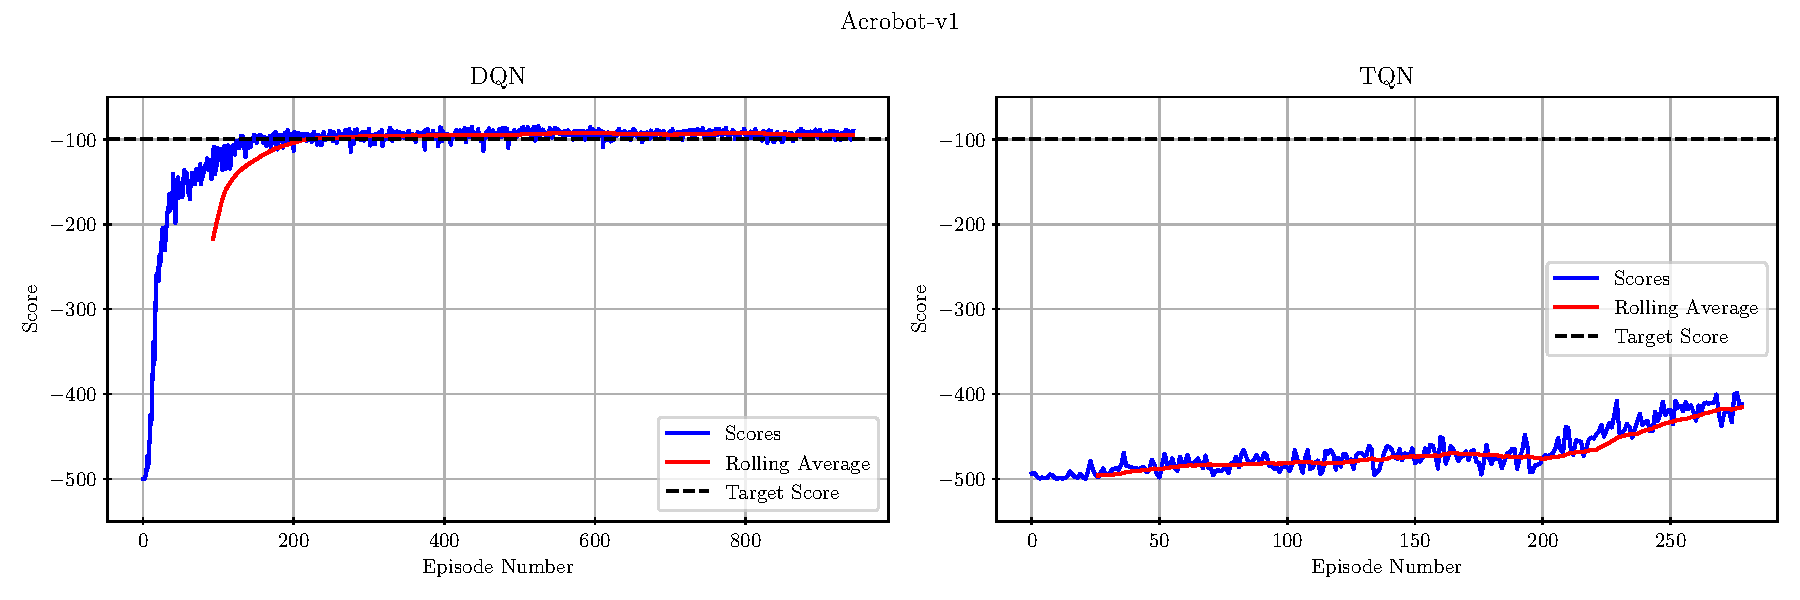
\includegraphics[width=\textwidth]{images/score-vs-episode_DQN-TQN_Acrobot-v1.pdf}
\caption{Score trend over time during training for Acrobot.}
\label{fig:score-vs-episode-Acrobot-v1}
\end{figure}

\begin{figure}[!htbp]
\centering
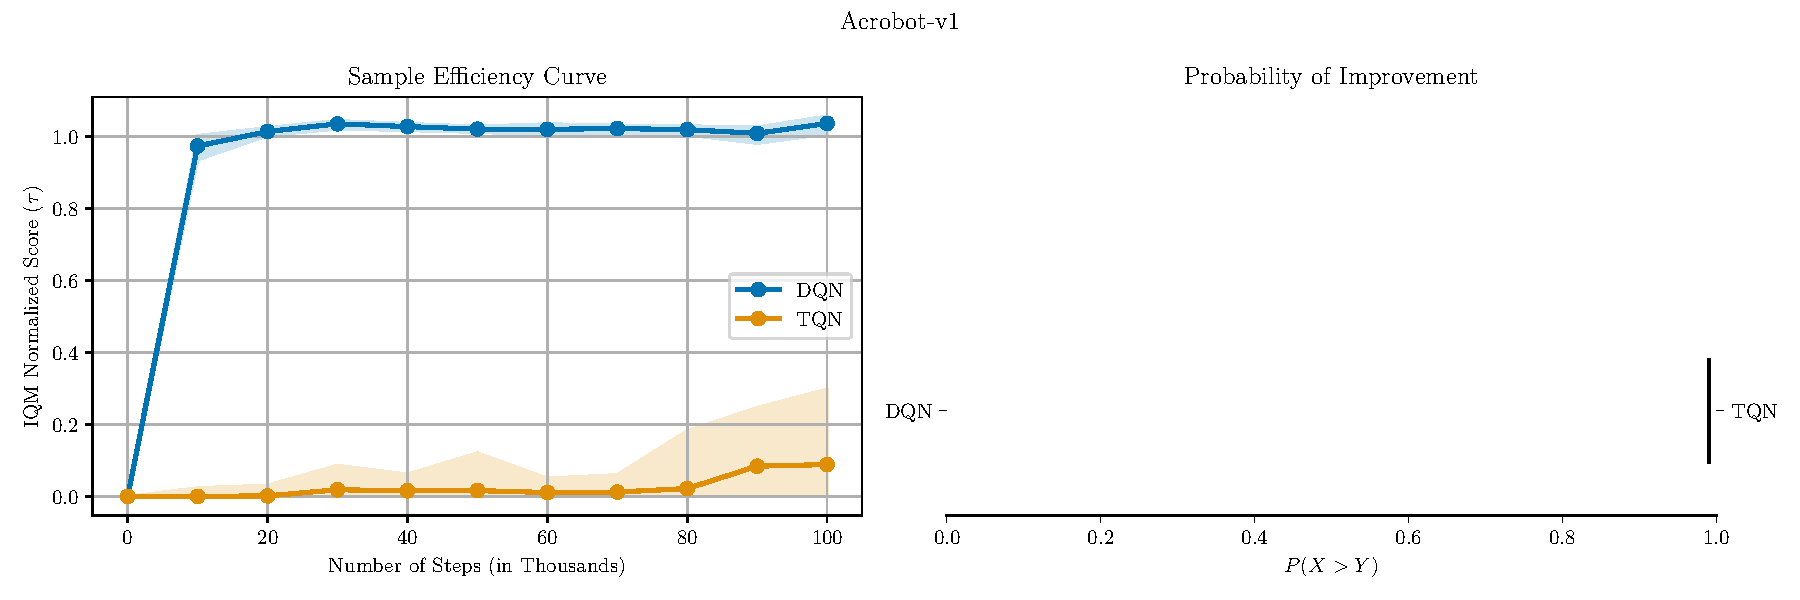
\includegraphics[width=\textwidth]{images/sample-efficiency-probability-improvement_DQN-TQN_Acrobot-v1.pdf}
\caption{Sample efficiency and probability of improvement for Acrobot.}
\label{fig:sample-efficiency-Acrobot-v1}
\end{figure}

\begin{figure}[!htbp]
\centering
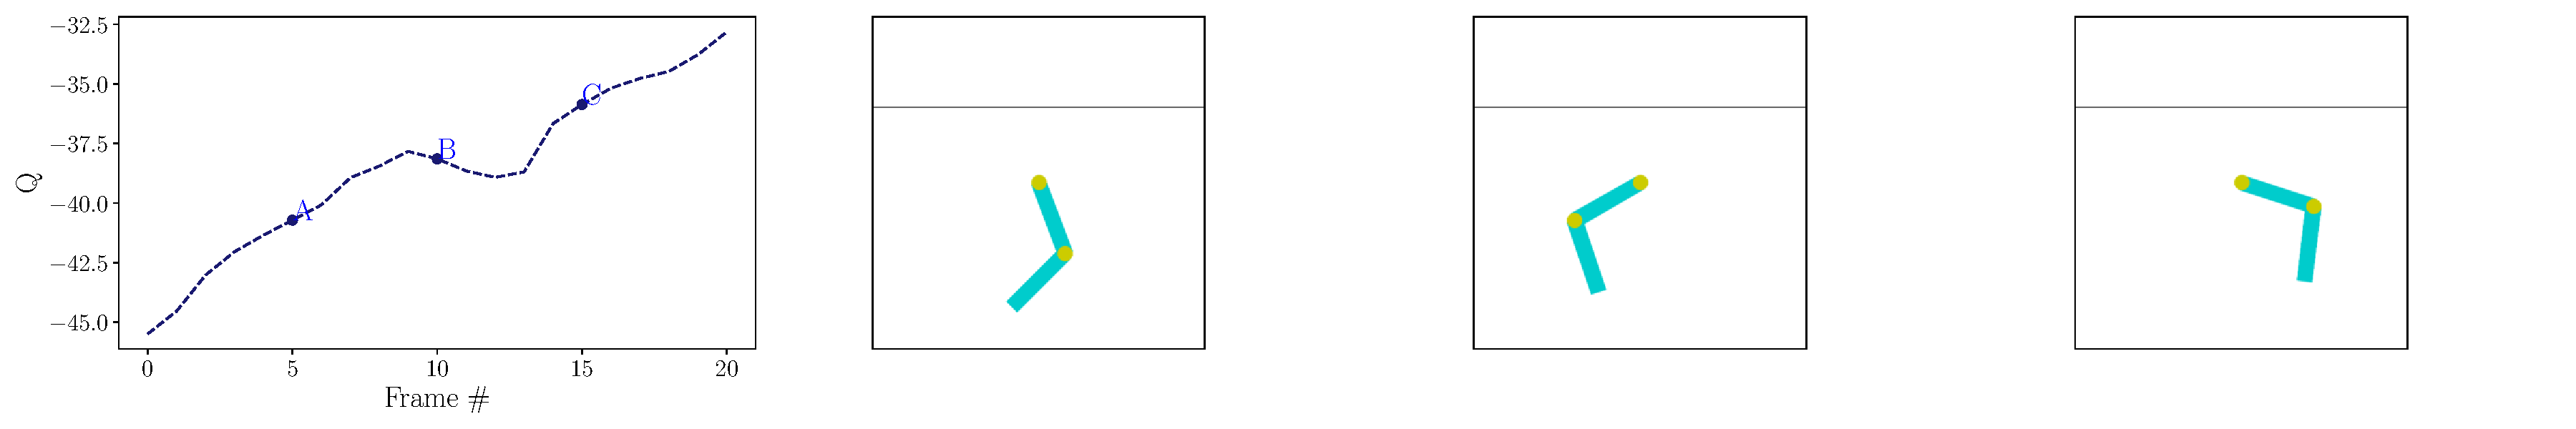
\includegraphics[width=\textwidth]{images/q-vs-frame_DQN_Acrobot-v1.pdf}
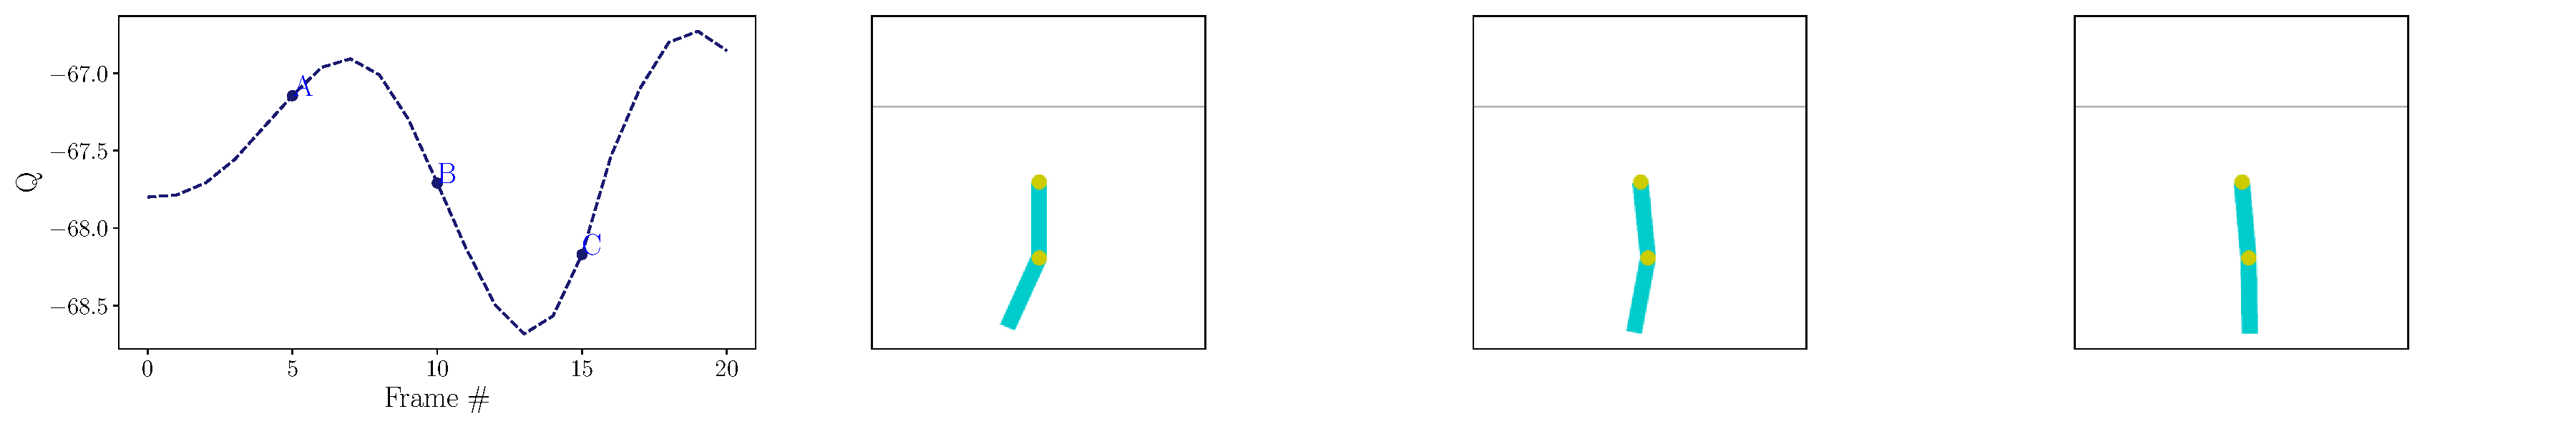
\includegraphics[width=\textwidth]{images/q-vs-frame_TQN_Acrobot-v1.pdf}
\caption{The predicted Q-values for a portion of a Acrobot episode and the three screenshots corresponding to frames A, B, and C. From top to bottom: \acrshort{dqn} and \acrshort{tqn}.}
\label{fig:q-vs-frame-DQN-Acrobot-v1}
\end{figure}

\begin{figure}[!htbp]
\centering
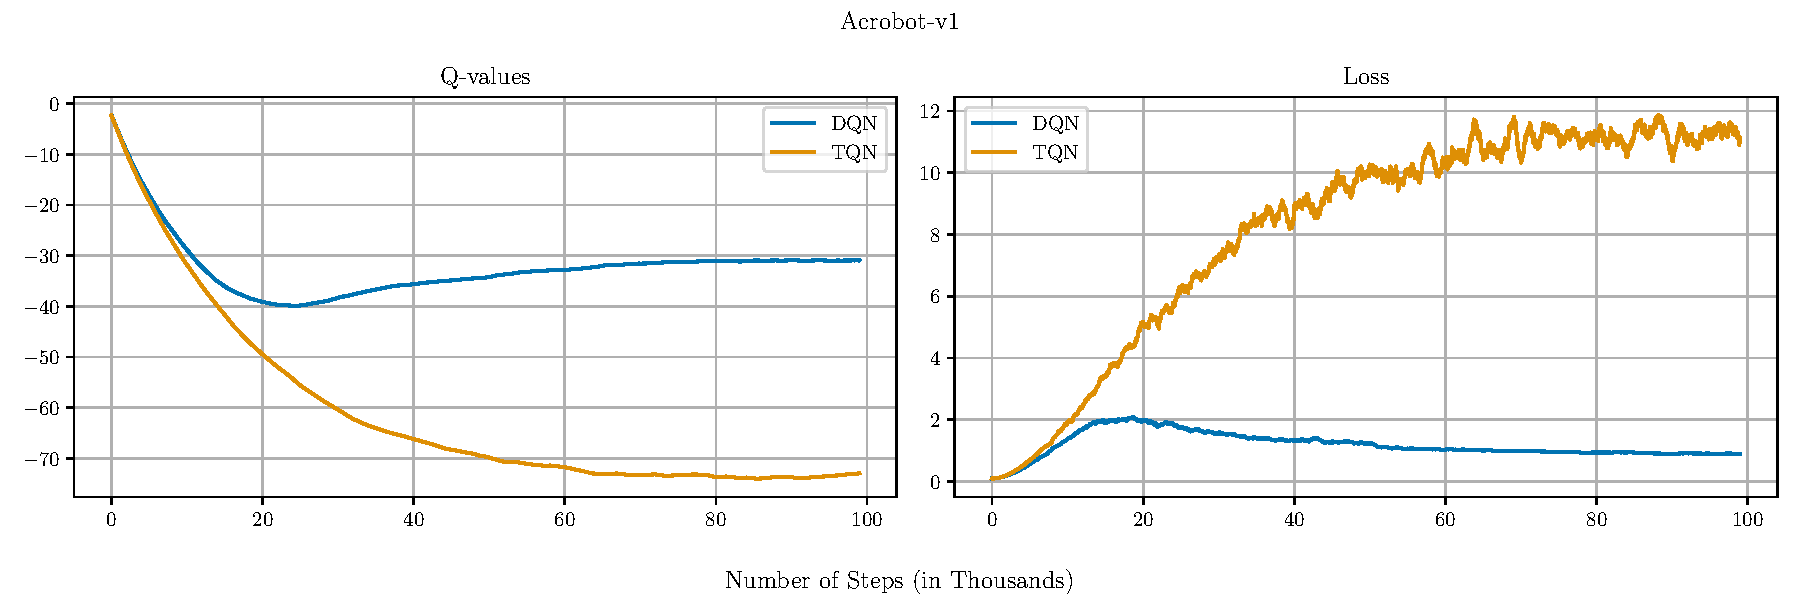
\includegraphics[width=\textwidth]{images/q-vs-loss_DQN-TQN_Acrobot-v1.pdf}
\caption{Q-values and loss over time for Acrobot.}
\label{fig:q-vs-loss-Acrobot=v1}
\end{figure}

\begin{figure}[!htbp]
\centering
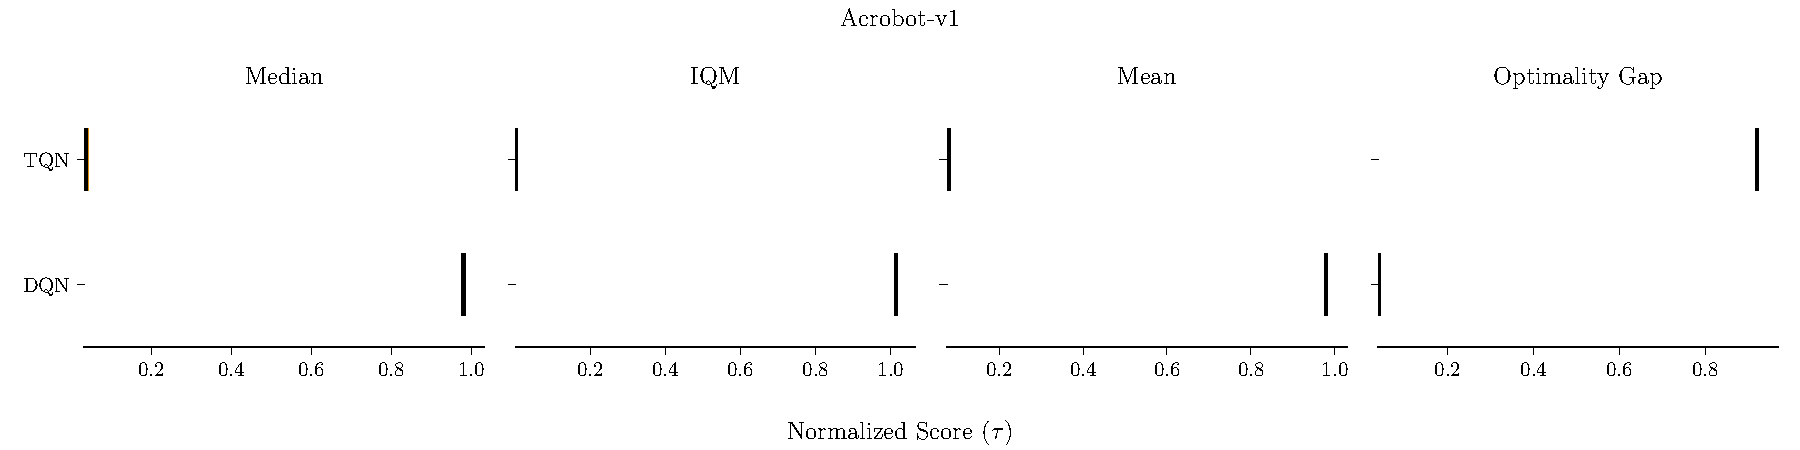
\includegraphics[width=\textwidth]{images/statistics_DQN-TQN_Acrobot-v1.pdf}
\caption{Median, \acrshort{iqm}, mean and optimality gap for Acrobot.}
\label{fig:statistics-Acrobot-v1}
\end{figure}

\subsection*{CartPole}
CartPole is widely regarded as one of the simplest environments, and yet no architecture was able to learn in the given amount of steps. There may be some differences with the implementation from which I borrow the hyperparameters \cite{rl_zoo3} that do not allow the agent to learn, or the hyperparameters are not really optimal and need further tuning. Time was limited though, and I was not able to further investigate the problem.

\begin{figure}[!htbp]
\centering
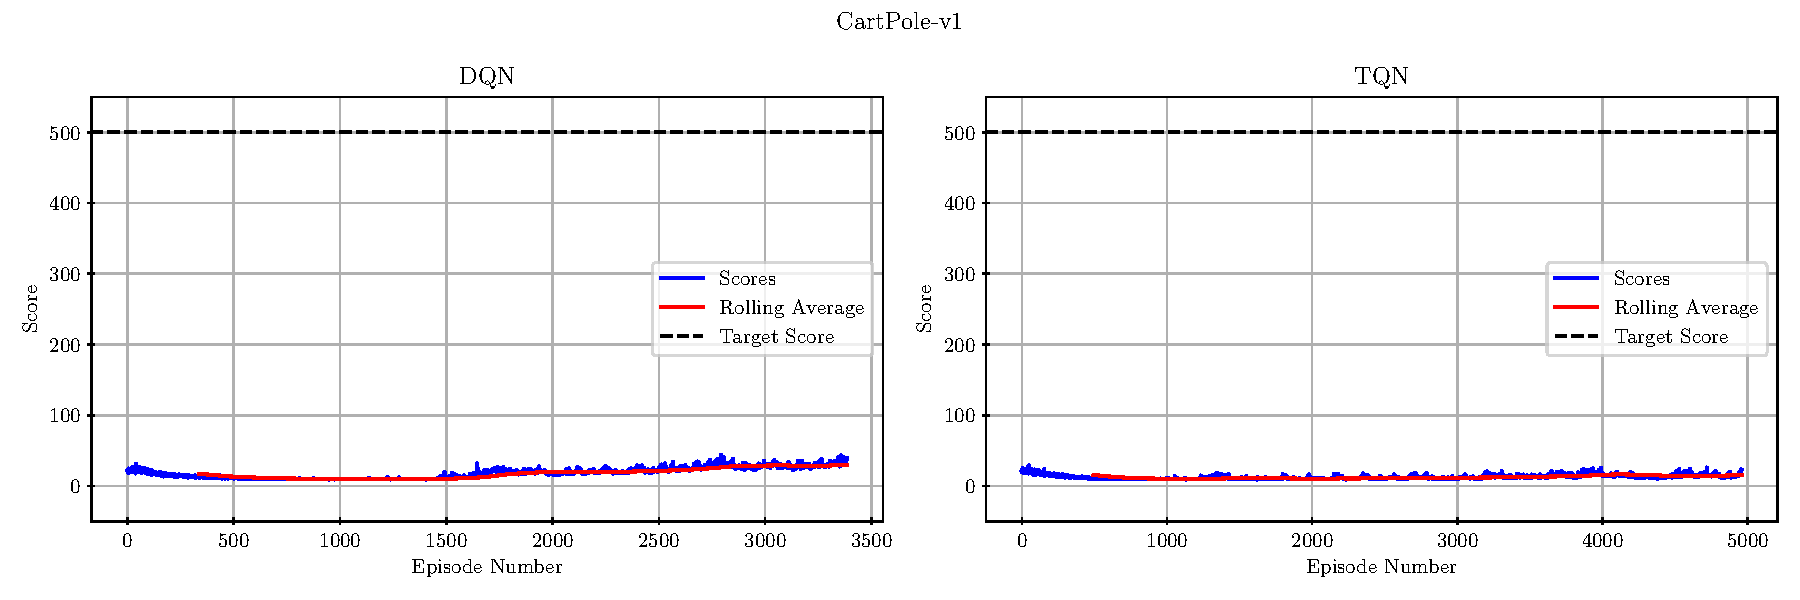
\includegraphics[width=\textwidth]{images/score-vs-episode_DQN-TQN_CartPole-v1.pdf}
\caption{Score trend over time during training for CartPole.}
\label{fig:score-vs-episode-CartPole-v1}
\end{figure}

\begin{figure}[!htbp]
\centering
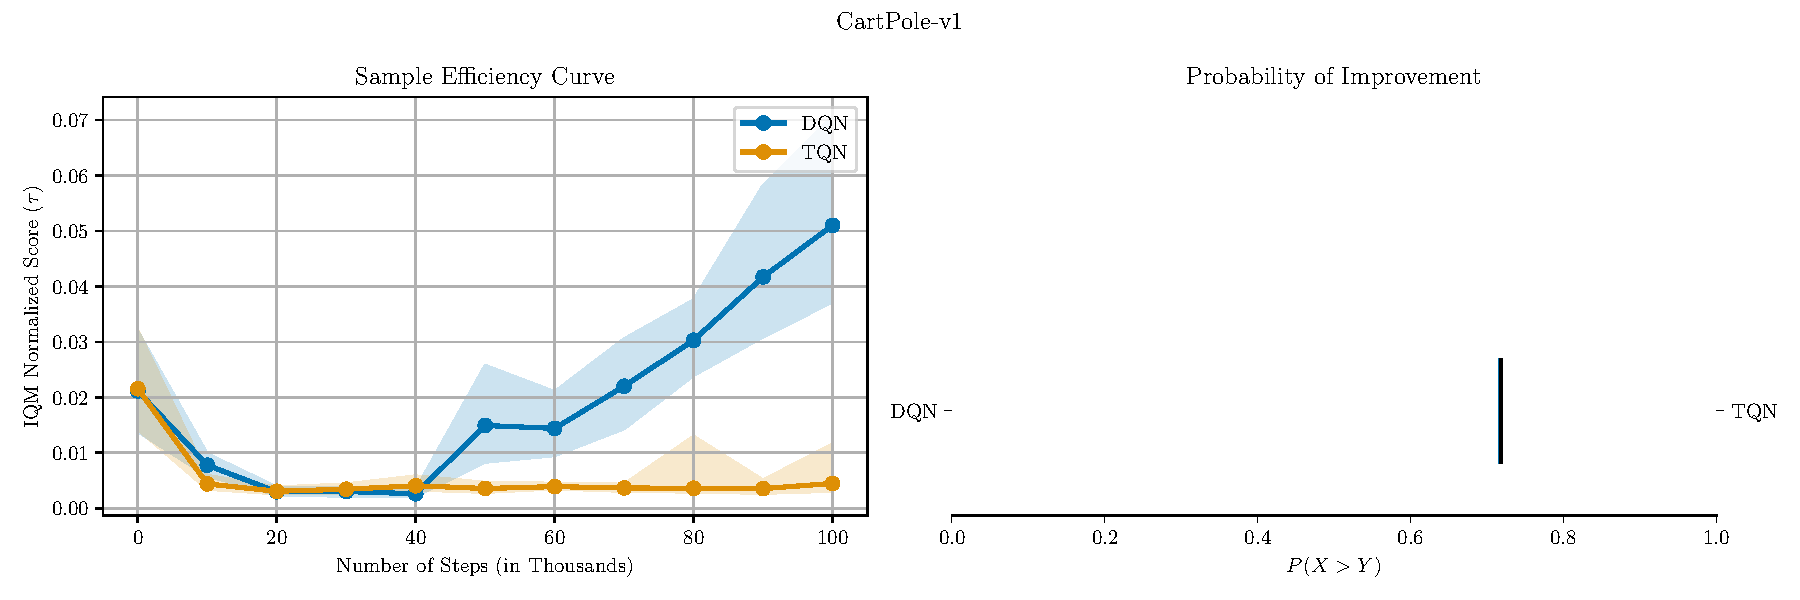
\includegraphics[width=\textwidth]{images/sample-efficiency-probability-improvement_DQN-TQN_CartPole-v1.pdf}
\caption{Sample efficiency and probability of improvement for CartPole.}
\label{fig:sample-efficiency-CartPole-v1}
\end{figure}

\begin{figure}[!htbp]
\centering
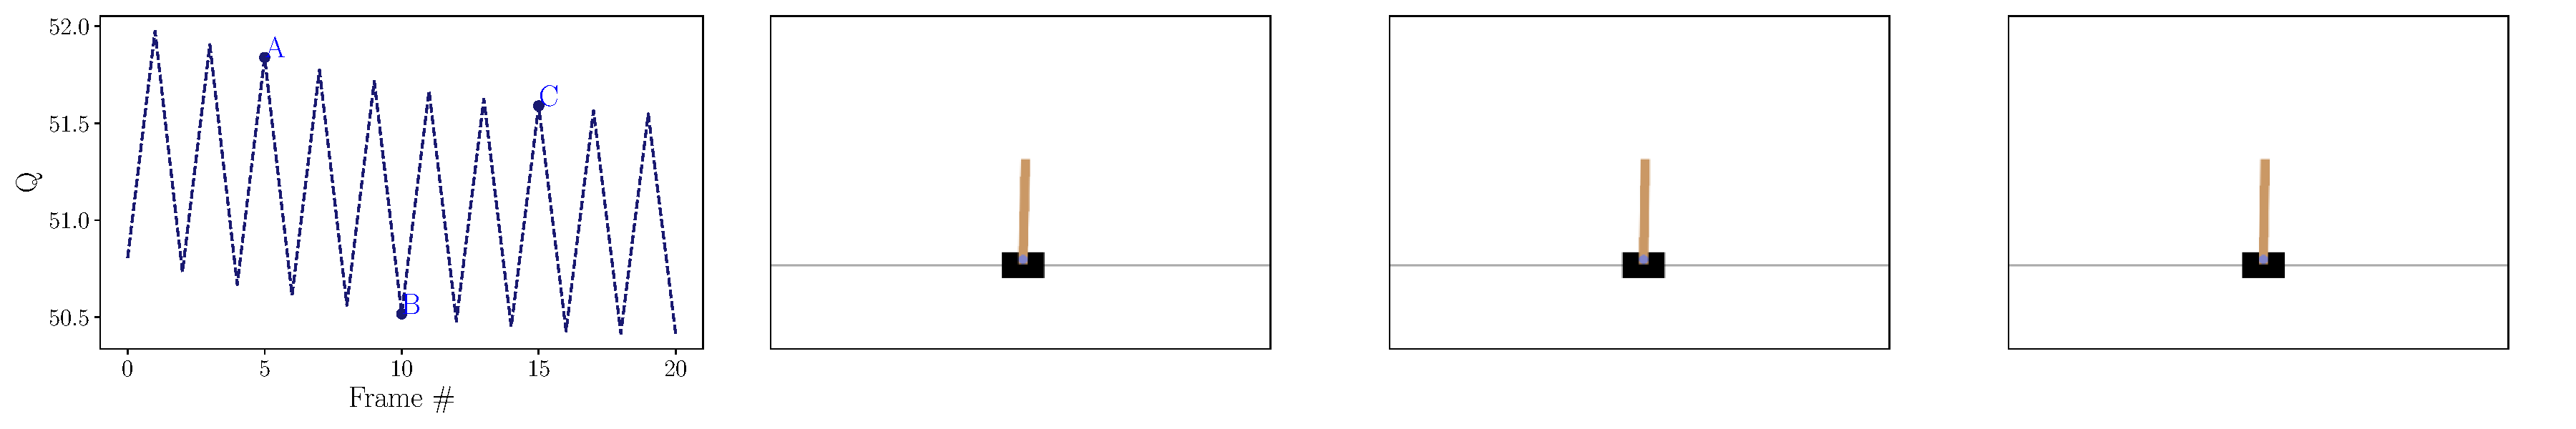
\includegraphics[width=\textwidth]{images/q-vs-frame_DQN_CartPole-v1.pdf}
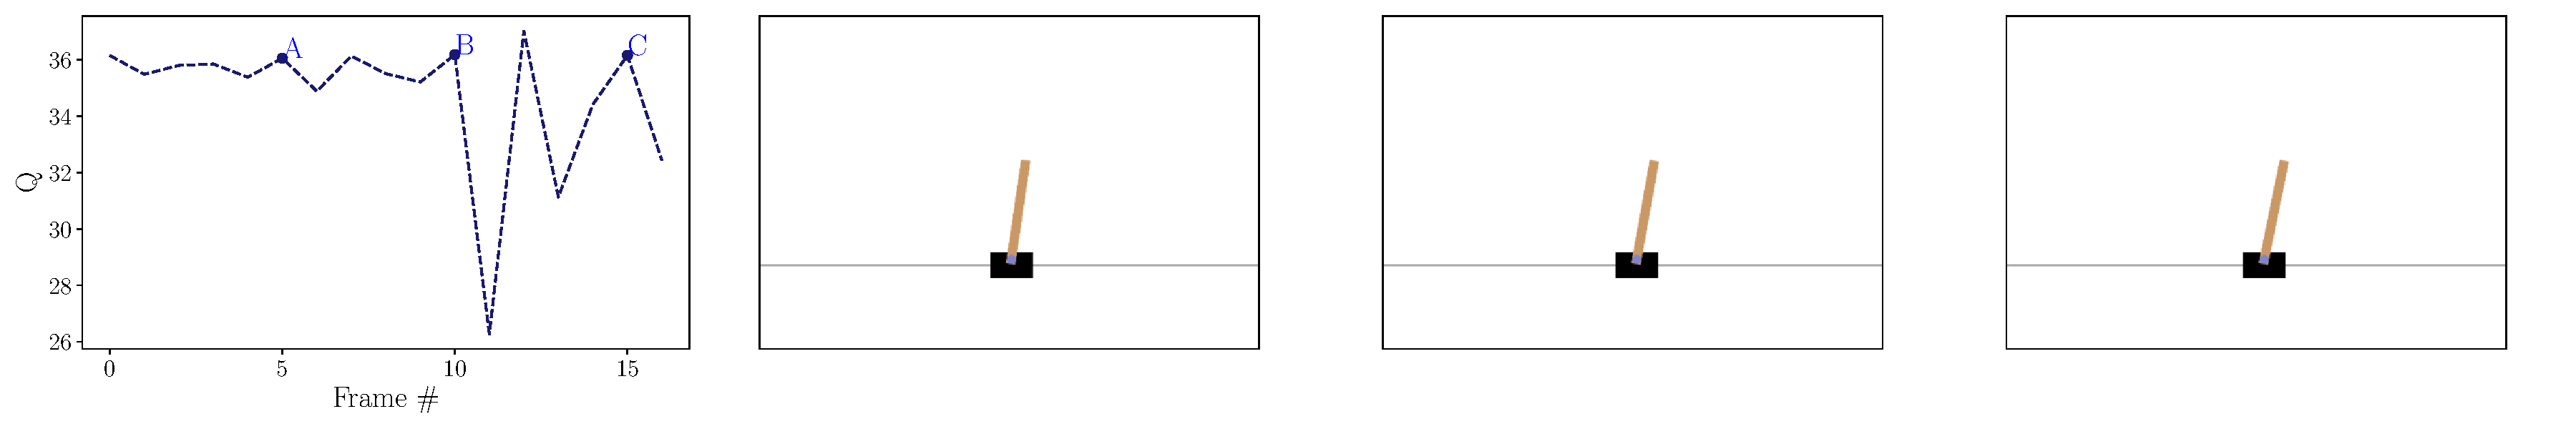
\includegraphics[width=\textwidth]{images/q-vs-frame_TQN_CartPole-v1.pdf}
\caption{The predicted Q-values for a portion of a CartPole episode and the three screenshots corresponding to frames A, B, and C. From top to bottom: \acrshort{dqn} and \acrshort{tqn}.}
\label{fig:q-vs-frame-DQN-CartPole-v1}
\end{figure}

\begin{figure}[!htbp]
\centering
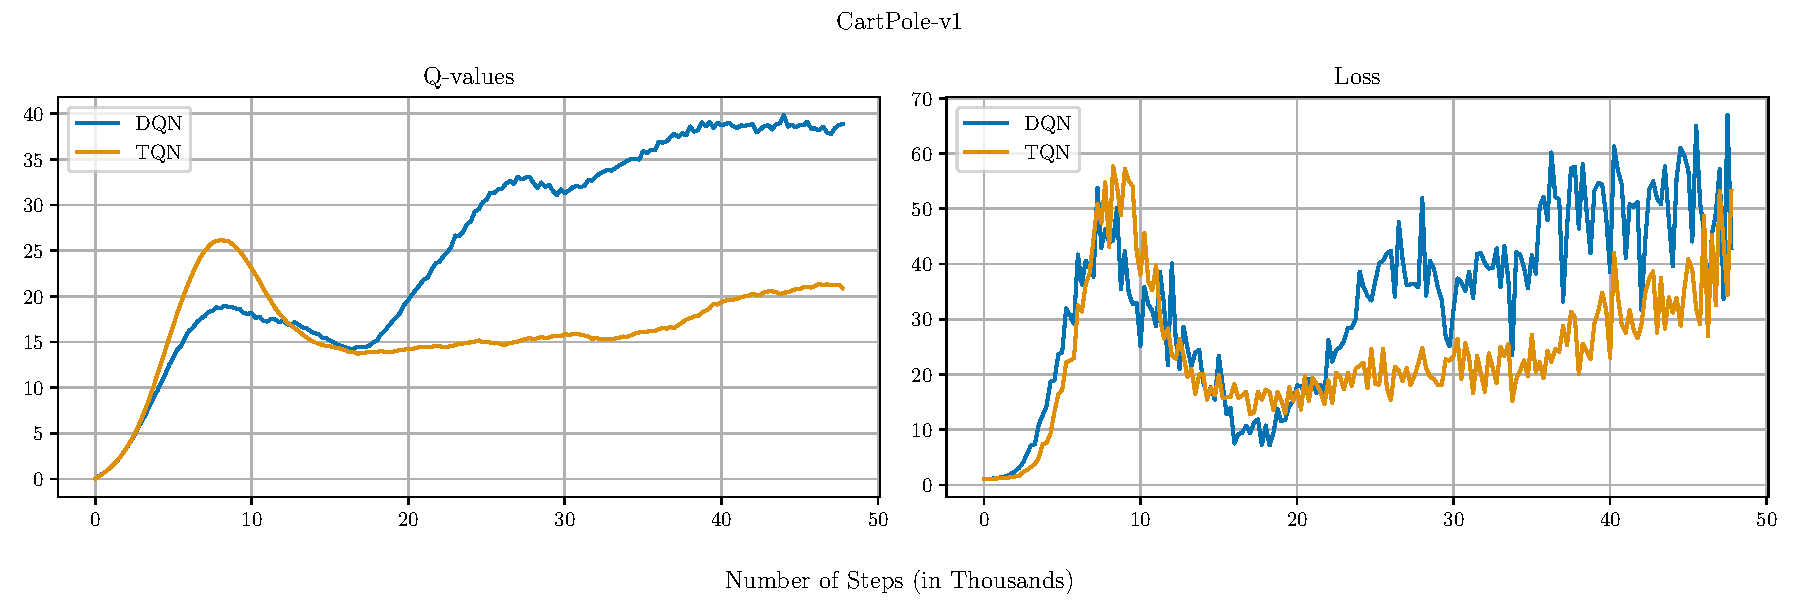
\includegraphics[width=\textwidth]{images/q-vs-loss_DQN-TQN_CartPole-v1.pdf}
\caption{Q-values and loss over time for CartPole.}
\label{fig:q-vs-loss-CartPole-v1}
\end{figure}

\begin{figure}[!htbp]
\centering
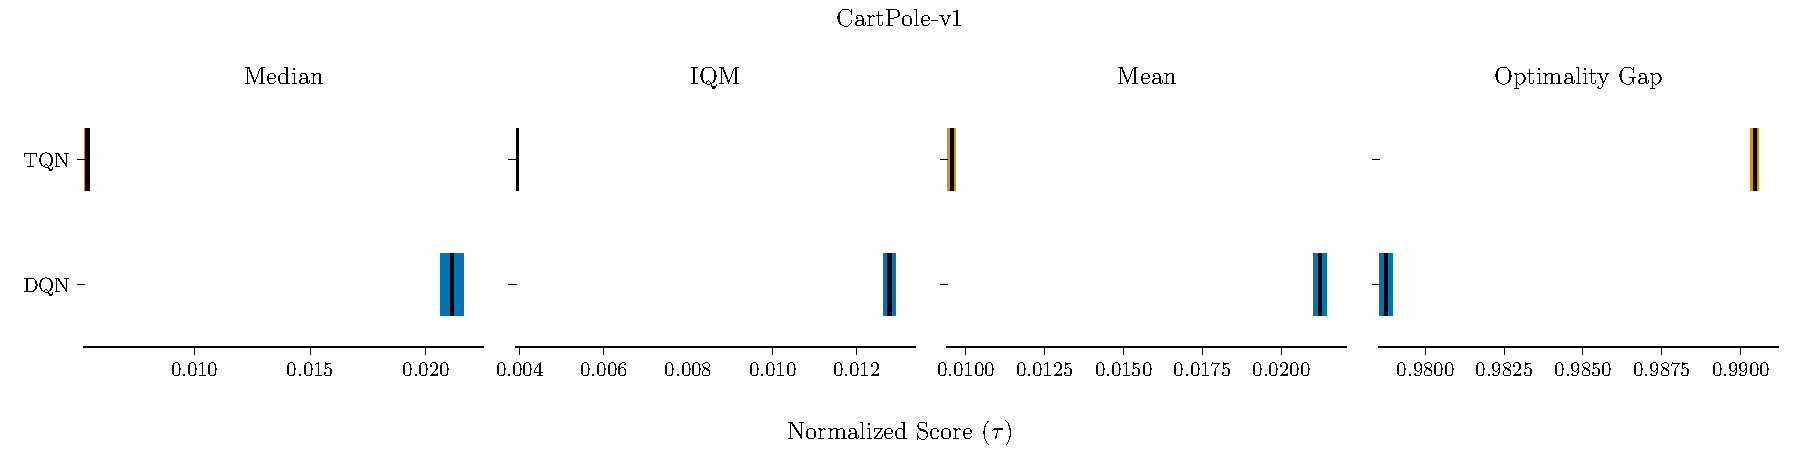
\includegraphics[width=\textwidth]{images/statistics_DQN-TQN_CartPole-v1.pdf}
\caption{Median, \acrshort{iqm}, mean and optimality gap for CartPole.}
\label{fig:statistics-CartPole-v1}
\end{figure}
